\documentclass{beamer}
\usetheme{CambridgeUS}
\usepackage[utf8]{inputenc}
\usepackage{graphicx}
\usepackage{tikz}

% Logo top-right
\logo{
\includegraphics[height=0.8cm]{HTL-logo.jpeg}} % Replace with correct path to HTL Anichstraße logo

% Title and author info
\title[AI Integration in Education and Dev]{Integration of Artificial Intelligence in Education and Software Development}
\author[Luna Sch\"atzle, Florian Prandstetter]{Luna Sch\"atzle \\ Florian Prandstetter}
\institute[HTL Anichstra\ss e]{HTL Anichstra\ss e, Department of Business Informatics\\Thesis Supervisor:\\Mag. Dr. Dipl. -Ing. Albert Greinöcker\\MMag.\textsuperscript{a} Eva-Maria Egger, MA}
\date{Diploma Thesis Defense -- April 2025}

\begin{document}

\begin{frame}
  \titlepage
\end{frame}

% Slide: Introduction
\begin{frame}{Introduction}
    \begin{itemize}
      \item \textbf{Presenter:} Luna Schätzle – Project Lead (AI evaluation, backend \& website)
      \item \textbf{Objective:} Open-source AI platform for education
      \item \textbf{Focus:} Evaluate various AI models for multiple use cases
      \item \textbf{Platform:} Enable students to access and experiment with AI
      \item \textbf{Motivation:} Overcome high resource requirements of current Open Source AI models
    \end{itemize}
  \end{frame}
  

% Slide: Project Team and Organization
%\begin{frame}{Project Team and Management}
%    \begin{itemize}
%      \item \textbf{Team Members:} Luna Schätzle, Florian Prandstetter
%      \item \textbf{Project Coordination:} Regular meetings, discussions, and planning sessions
%      \item \textbf{Tools Employed:}
%        \begin{itemize}
%          \item GitHub for version control and collaborative coding
%          \item Discord for communication and coordination
%          \item Google Sheets for time tracking
%          \item LaTeX for comprehensive documentation
%        \end{itemize}
%    \end{itemize}
%  \end{frame}
  
% Slide: Theoretical Background
%\begin{frame}{Theoretical Background}
%    \begin{itemize}
%      \item \textbf{LLMs Integration:} Evaluation and incorporation of various Large Language Models.
%      \item \textbf{Interfaces:} API connections, local models (e.g., Ollama), and OpenAI API.
%      \item \textbf{Evaluation:} Systematic testing of open source models 
%    \end{itemize}
%  \end{frame}

\begin{frame}{Open Source: Impact \& Approach}
  \begin{itemize}
    \item \textbf{Definition:} Public, collaborative development
    \item \textbf{Benefits:} Cost-efficient, flexible, secure via community review
    \item \textbf{Impact:} Fuels innovation and startup growth
    \item \textbf{Our Approach:} Leveraging Python, Flask, Vue.js 
    \item \textbf{Our Application:} Open-source licensed under GNU GPL-3.0
  \end{itemize}
\end{frame}

  

% Slide: Testing and Evaluation
\begin{frame}{Testing and Evaluation}
  \begin{itemize}
    \item Evaluation of models: Llama3.2, Deepseek-r1, gemma2, qwen, ...
    \item Testing methods: Different prompts and tasks where asked the models (automated via Python script)
    \item Evaluation criteria: 
      \begin{itemize}
        \item response time
        \item accuracy
        \item resource usage
        \item BLEU score
        \item readability
        \item Textquality
      \end{itemize}
  \end{itemize}
\end{frame}

\begin{frame}{Evaluation Results}
  \begin{itemize}
    \item \textbf{Data Preparation:} Graphical analysis was conducted to elucidate patterns.
    \item \textbf{Model Performance:}
      \begin{itemize}
        \item Marked differences in response time, accuracy, and resource consumption.
        \item Smaller models demonstrated superior efficiency.
      \end{itemize}
    \item \textbf{User Integration:}
      \begin{itemize}
        \item A diverse array of models is available for selection.
        \item The top-performing model is auto-recommended.
      \end{itemize}
    \item \textbf{Key Insight:} Model size does not reliably predict quality; balanced assessments are imperative.
  \end{itemize}
\end{frame}


% Slide: Backend Architecture
%\begin{frame}{Backend Architecture}
%  \begin{itemize}
%    \item Design based on model integration needs
%    \item Functionality of the backend (AI Hub, Code Bot)
%    \item Structure: Flask-based API, endpoints for services
%    \item Reference to server setup by Florian
%  \end{itemize}
%\end{frame}

\begin{frame}{Website Platform}
  \begin{itemize}
    \item Developed to make AI accessible to students.
    \item Built with:
    \begin{itemize}
      \item Vue.js (Frontend)
      \item Flask (Backend API)
      \item Firebase (User data \& authentication)
    \end{itemize}
    \item Purpose: Central interface for interacting with various AI tools.
  \end{itemize}
  \vspace{0.5cm}
  \centering
  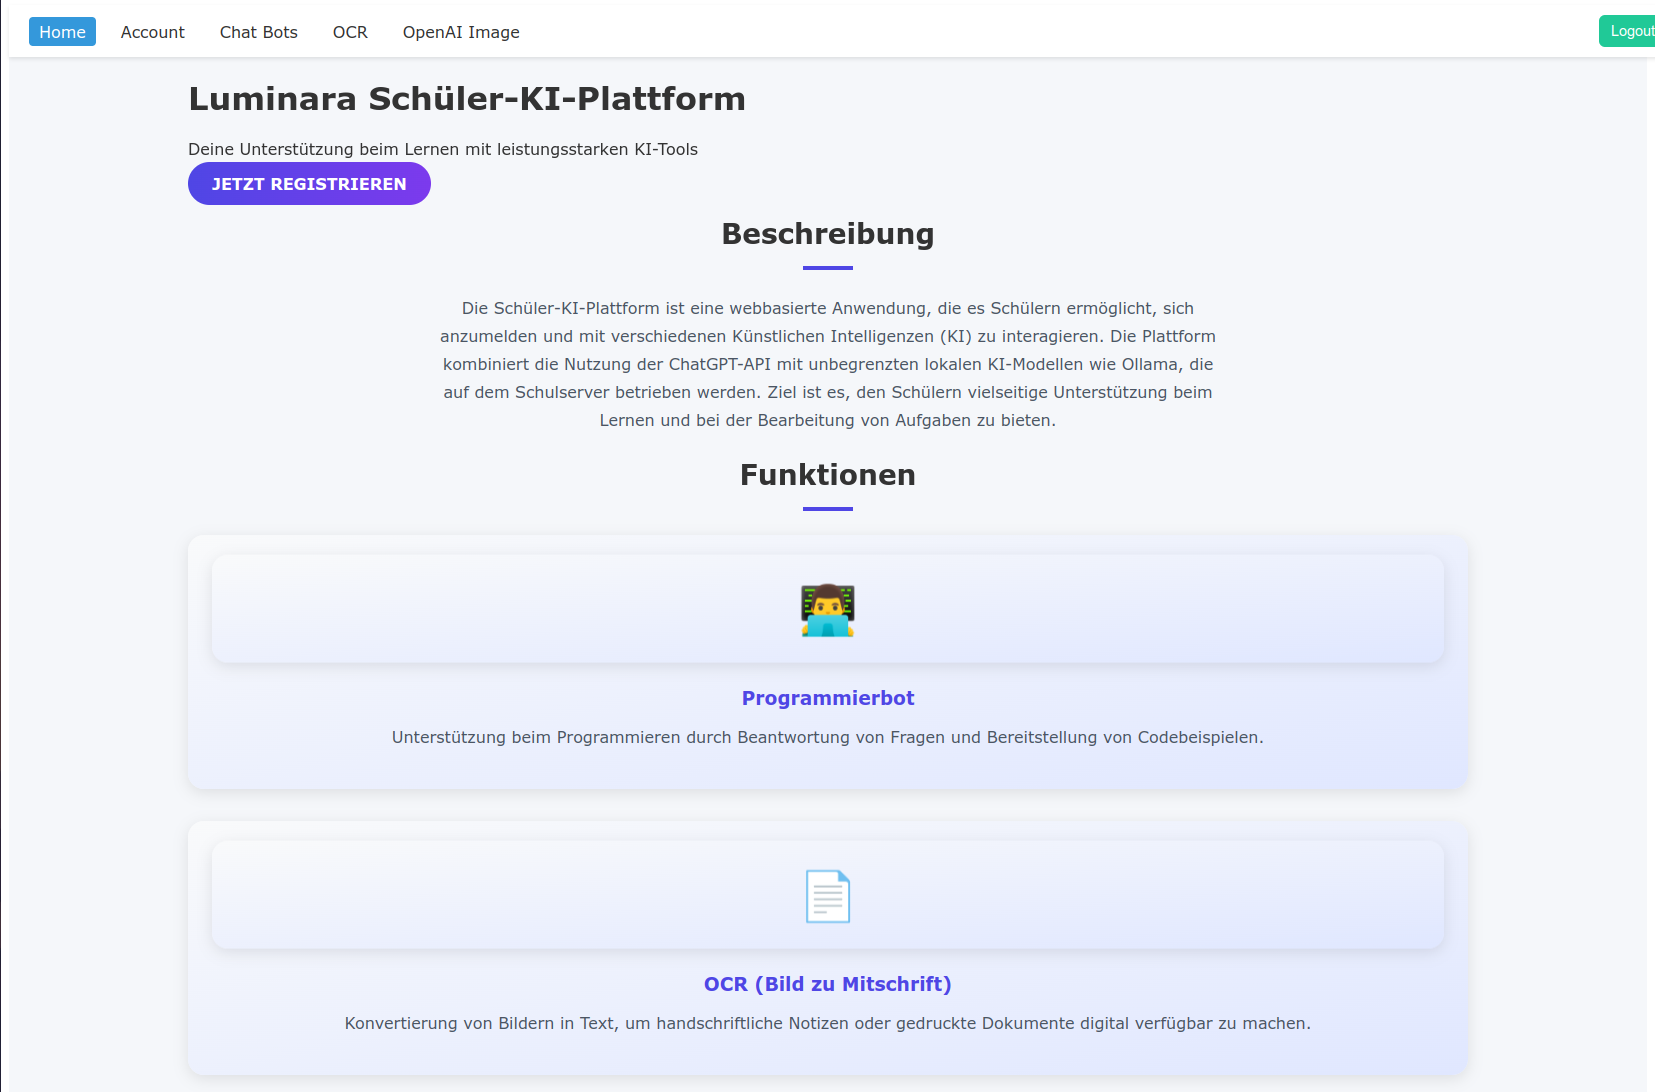
\includegraphics[height=3.5cm]{homepage-screenshot.png} % ← Screenshot of homepage
\end{frame}



\begin{frame}{User System}
  \begin{itemize}
    \item Registration and secure login
    \item Profile management
    \item Firebase-based authentication
  \end{itemize}
  \vspace{0.5cm}
  \centering
  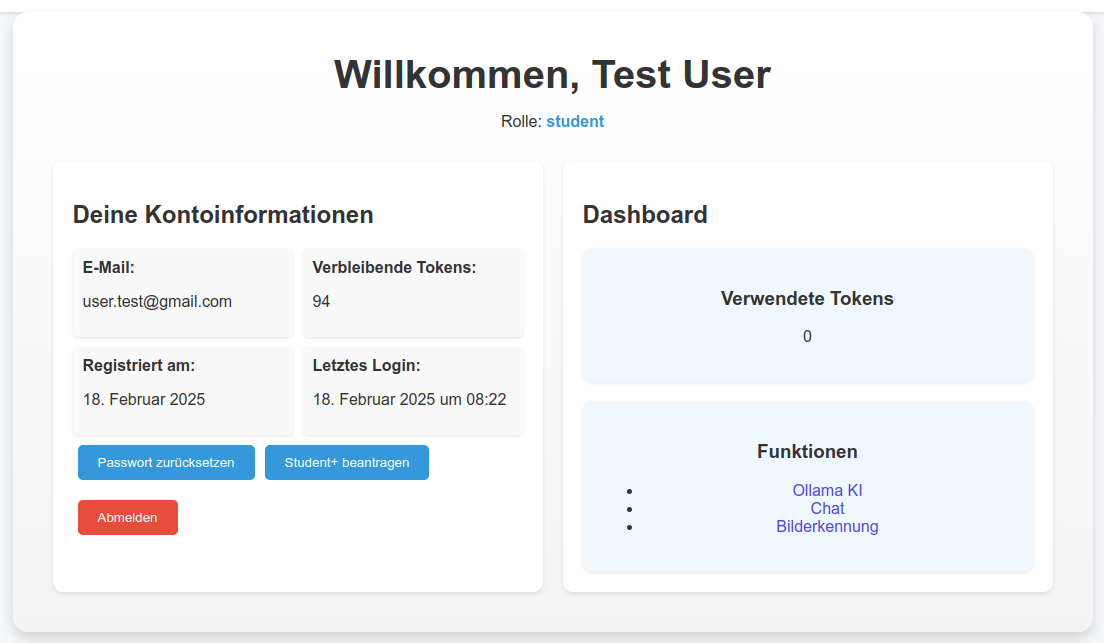
\includegraphics[height=3.5cm]{Account-Managment.png} % ← Screenshot: Login/Registration
\end{frame}

\begin{frame}{Chatbot Interface}
  \begin{itemize}
    \item Multiple AI models available via tabs:
    \begin{itemize}
      \item ChatGPT (OpenAI API)
      \item Local models (e.g., Ollama)
      \item Programming Assistant
    \end{itemize}
    \item Vision models: LLaVA, LLaMA 3.2 Vision
  \end{itemize}
  \vspace{0.5cm}
  \centering
  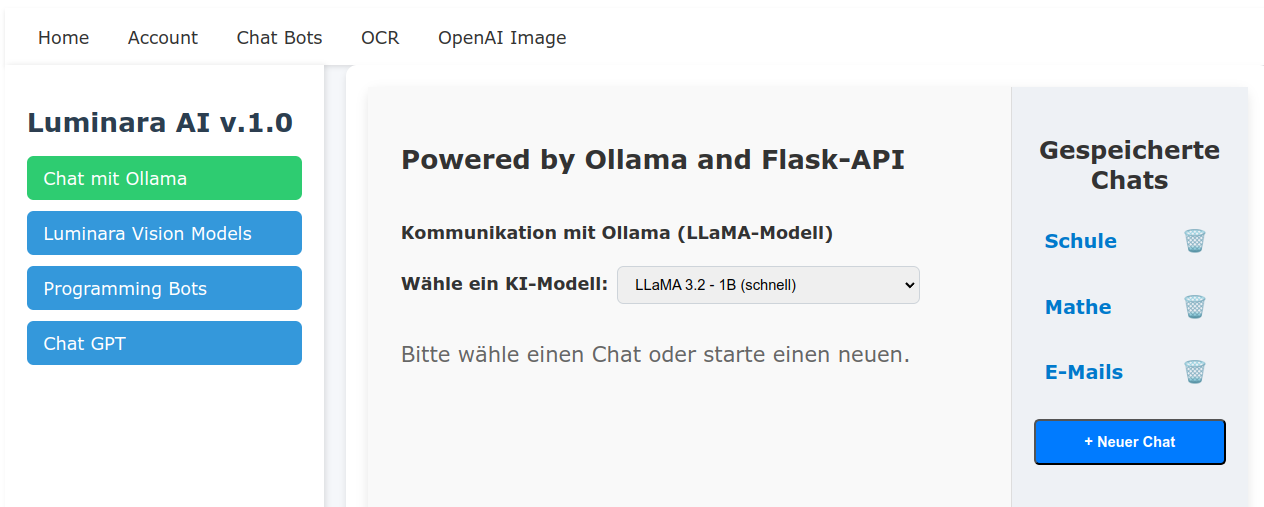
\includegraphics[height=3.5cm]{Chat-Bot-Navigation-Bar.png} % ← Screenshot of chatbot interface
\end{frame}

\begin{frame}{Image Generation}
  \begin{itemize}
    \item Generate images from text prompts
    \item Uses DALL·E (OpenAI)
  \end{itemize}
  \vspace{0.5cm}
  \centering
  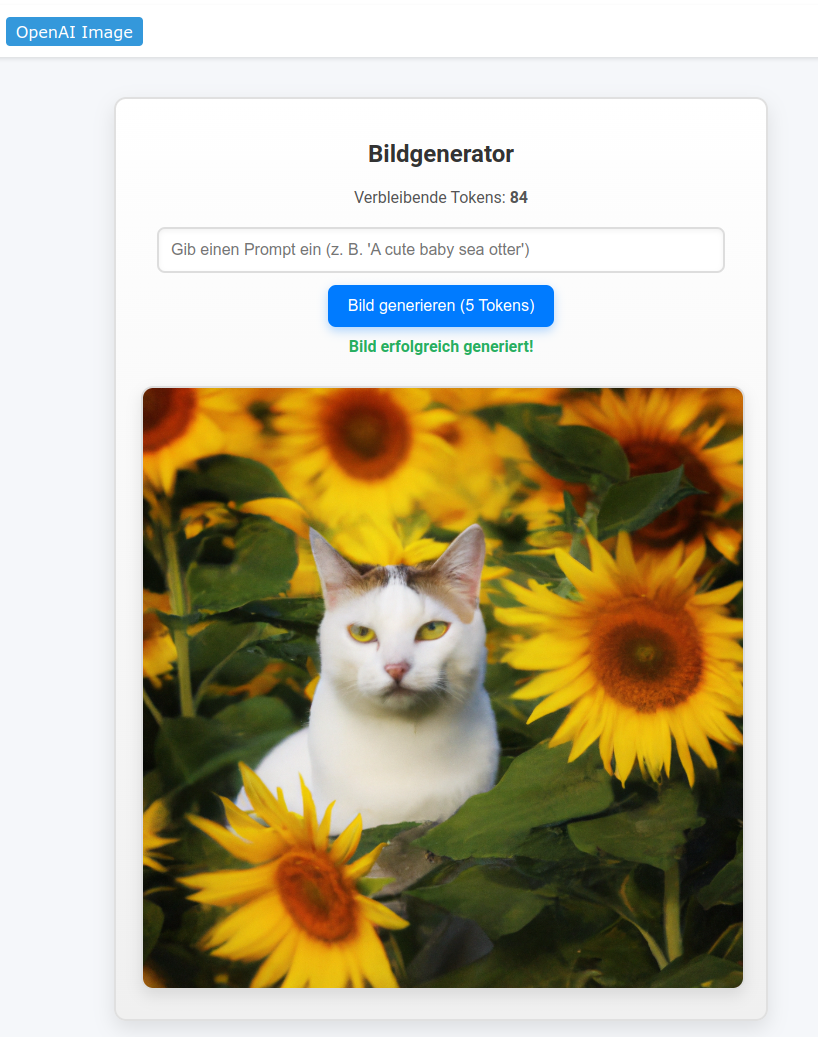
\includegraphics[height=5cm]{image-generation.png} % ← Screenshot of image generation
\end{frame}

\begin{frame}{OCR and Image Recognition}
  \begin{itemize}
    \item OCR with Tesseract
    \item Post-processing using a large language model
    \item Leverages Markdown for formatting
  \end{itemize}
  \vspace{0.5cm}
  \centering
  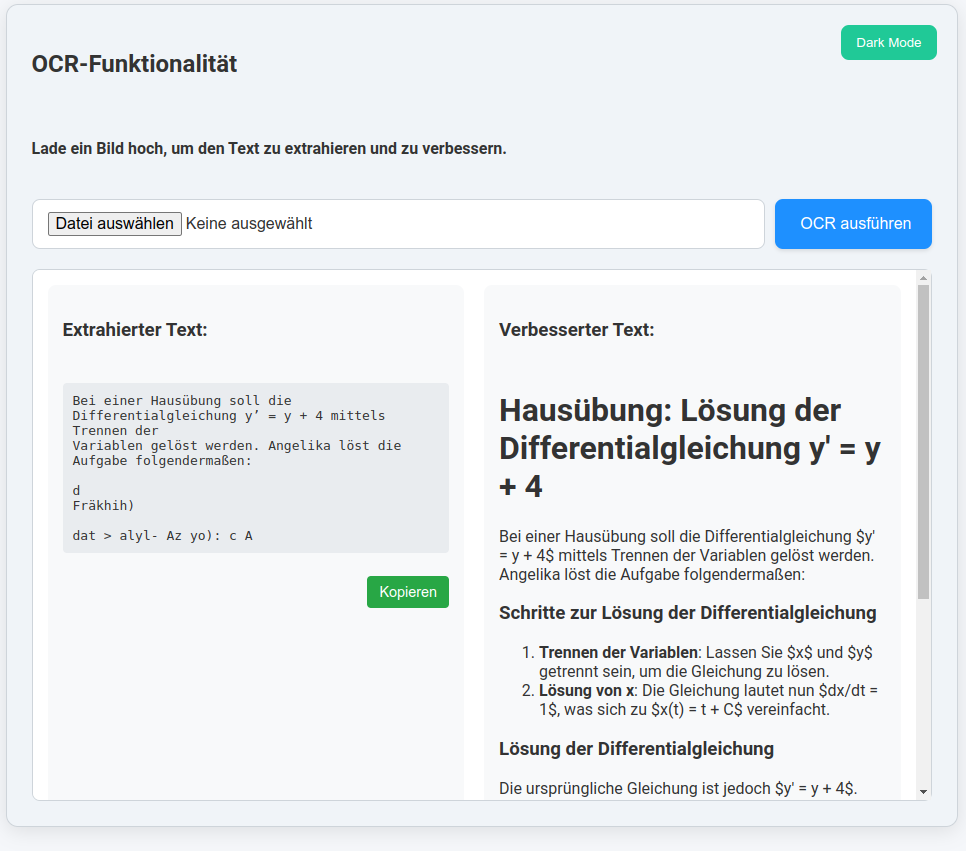
\includegraphics[height=3.5cm]{OCR-functonalatie.png} % ← Screenshot OCR feature
\end{frame}


% Slide: AI in Economics and Ethics
\begin{frame}{AI in Economics and Ethics}
\textbf{Applications:}
        \begin{itemize}
          \item Customer service \& support
          \item Supply chain management
          \item Predictive analytics
          \item Data analysis
          \item Process automation
        \end{itemize}

\end{frame}

% Slide: AI in Economics and Ethics
\begin{frame}{AI in Economics and Ethics}
\textbf{Ethical \& Social Concerns:}
        \begin{itemize}
          \item Bias in training data
          \item Transparency \& accountability
          \item Privacy and data protection
          \item Impact on the workflow and job displacements
        \end{itemize}
\end{frame}

% Slide: AI in Economics and Ethics
\begin{frame}{AI in Economics and Ethics}
\textbf{Regulatory Challenges:}
            \begin{itemize}
              \item Data security standards (e.g., GDPR [EUR-Lex: 2016/679])
              \item EU AI Act considerations [EUR-Lex: 2024/1689]
              \item Inconsistent global regulations 
            \end{itemize}
\end{frame}



% Slide: Conclusion
%\begin{frame}{Conclusion}
%  \begin{itemize}
%    \item Summary of achievements
%    \item Insights gained during the development
%    \item Future potential of the system
%    \item Final thoughts and acknowledgments
%  \end{itemize}
%\end{frame}

\begin{frame}[plain]
  % Background HTL logo with transparency
  \begin{tikzpicture}[remember picture,overlay]
    \node[opacity=0.2] at (current page.center) 
      {
\includegraphics[width=0.6\paperwidth]{HTL-logo.jpeg}};
  \end{tikzpicture}
  
  \centering
  \vspace{1cm}
  \Huge Thank You for Your Attention!
\end{frame}

\begin{frame}[plain]
  % Background HTL logo with transparency
  \begin{tikzpicture}[remember picture,overlay]
    \node[opacity=0.2] at (current page.center) 
      {
\includegraphics[width=0.6\paperwidth]{HTL-logo.jpeg}};
  \end{tikzpicture}
  
  \centering
  \vspace{1cm}
  \Huge Backup slides Graphics
\end{frame}

%backup Slides for possible Questions
%Maby extra slide with the results
\begin{frame}{Evaluation Results: Qualitative metrics}
  \begin{figure}
    \centering
    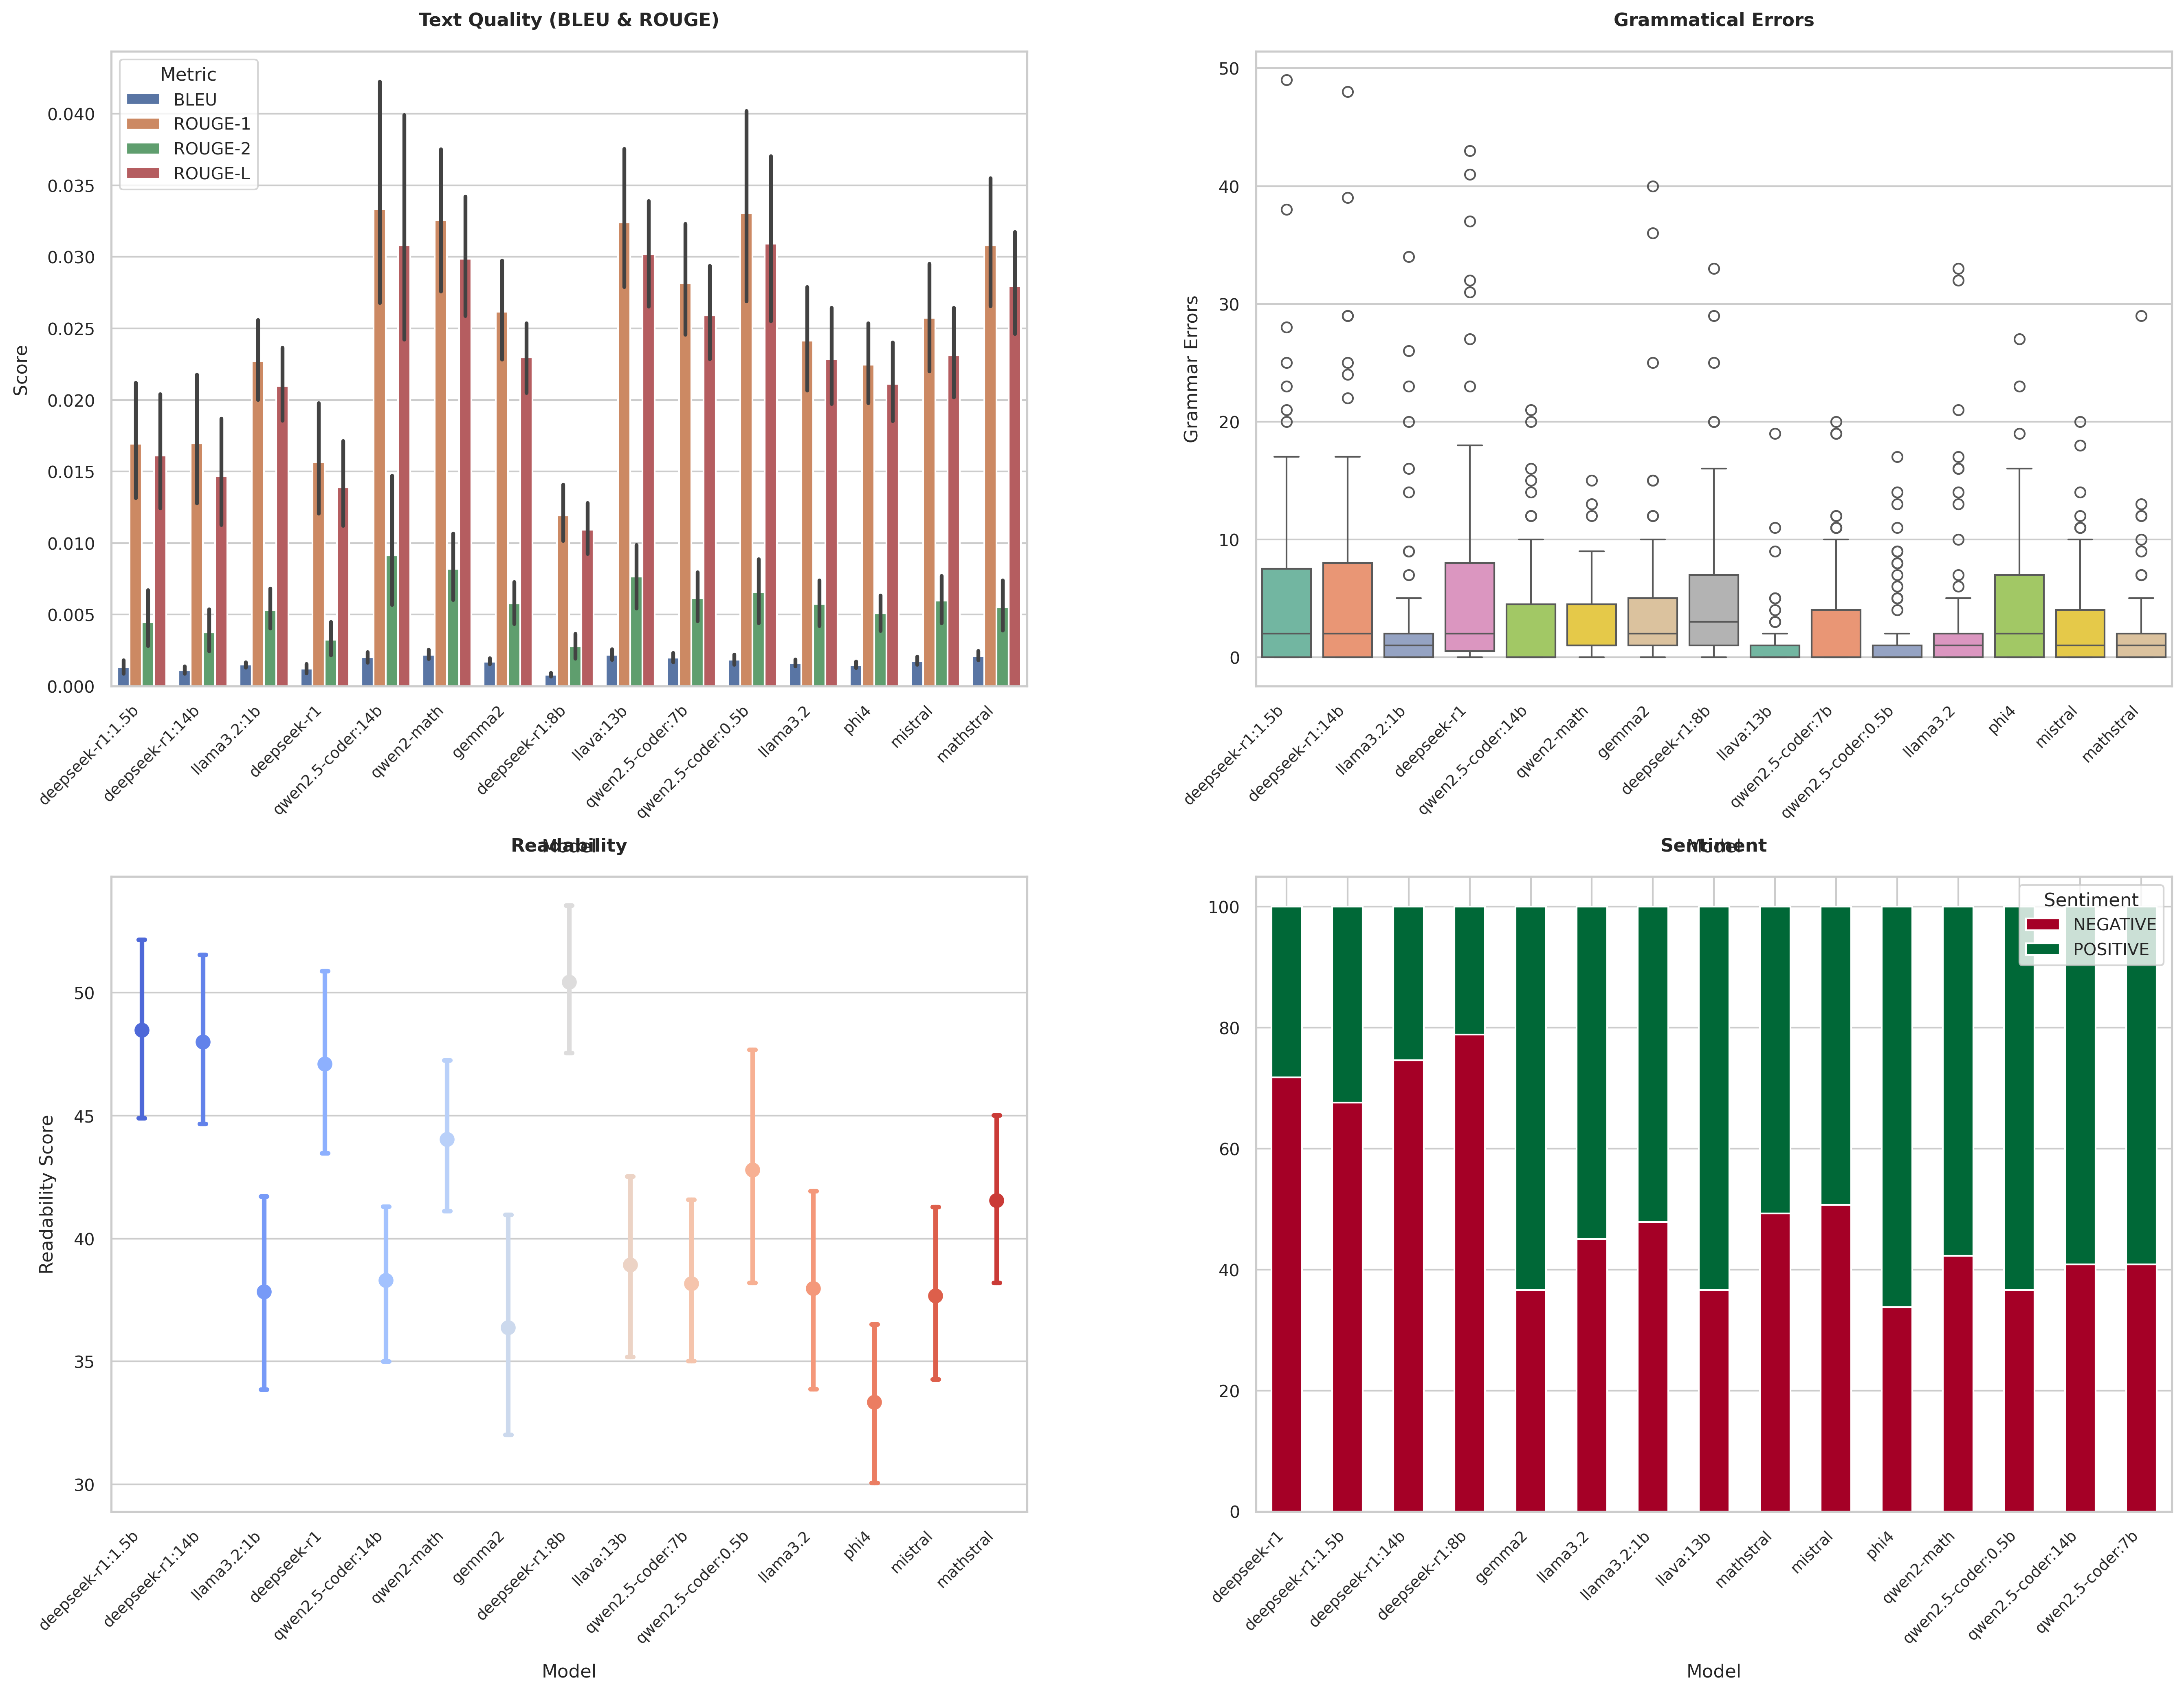
\includegraphics[width=0.8\textwidth]{combined_metrics.png}
    \caption{Evaluation Results of AI Models}
    \label{fig:evaluation-results}
  \end{figure}
\end{frame}

\begin{frame}{Evaluation Results: Quantitative metrics}
  \begin{columns}[t]
    \column{0.5\textwidth}
      \begin{figure}
        \centering
        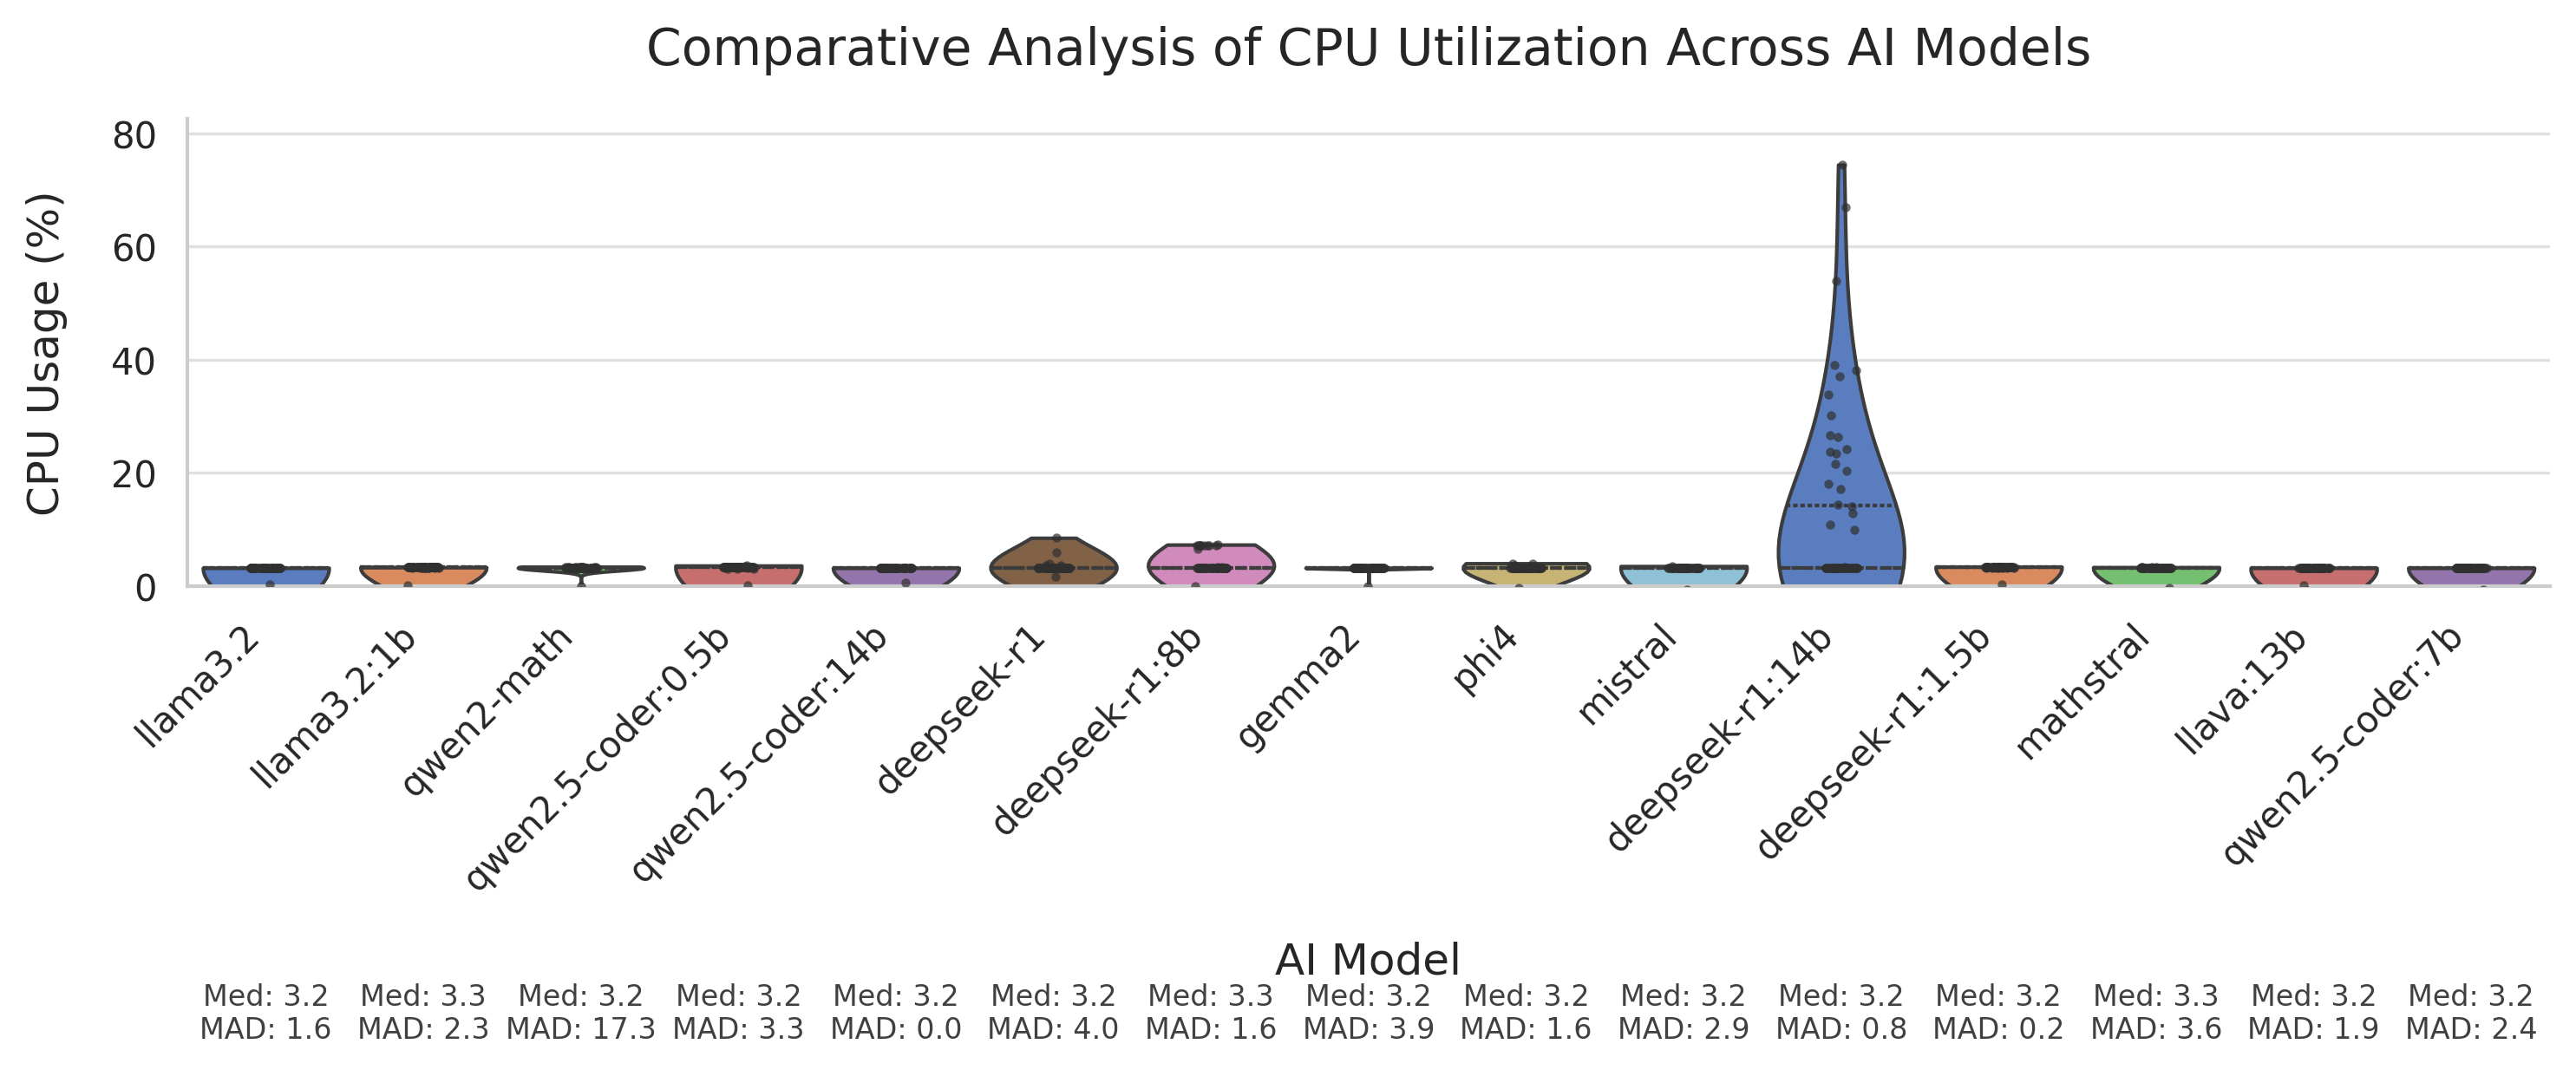
\includegraphics[width=0.9\columnwidth]{model_cpu_usage_comparison.png}
        \caption{CPU Usage Comparison}
        \label{fig:cpu-usage}
      \end{figure}
    \column{0.5\textwidth}
      \begin{figure}
        \centering
        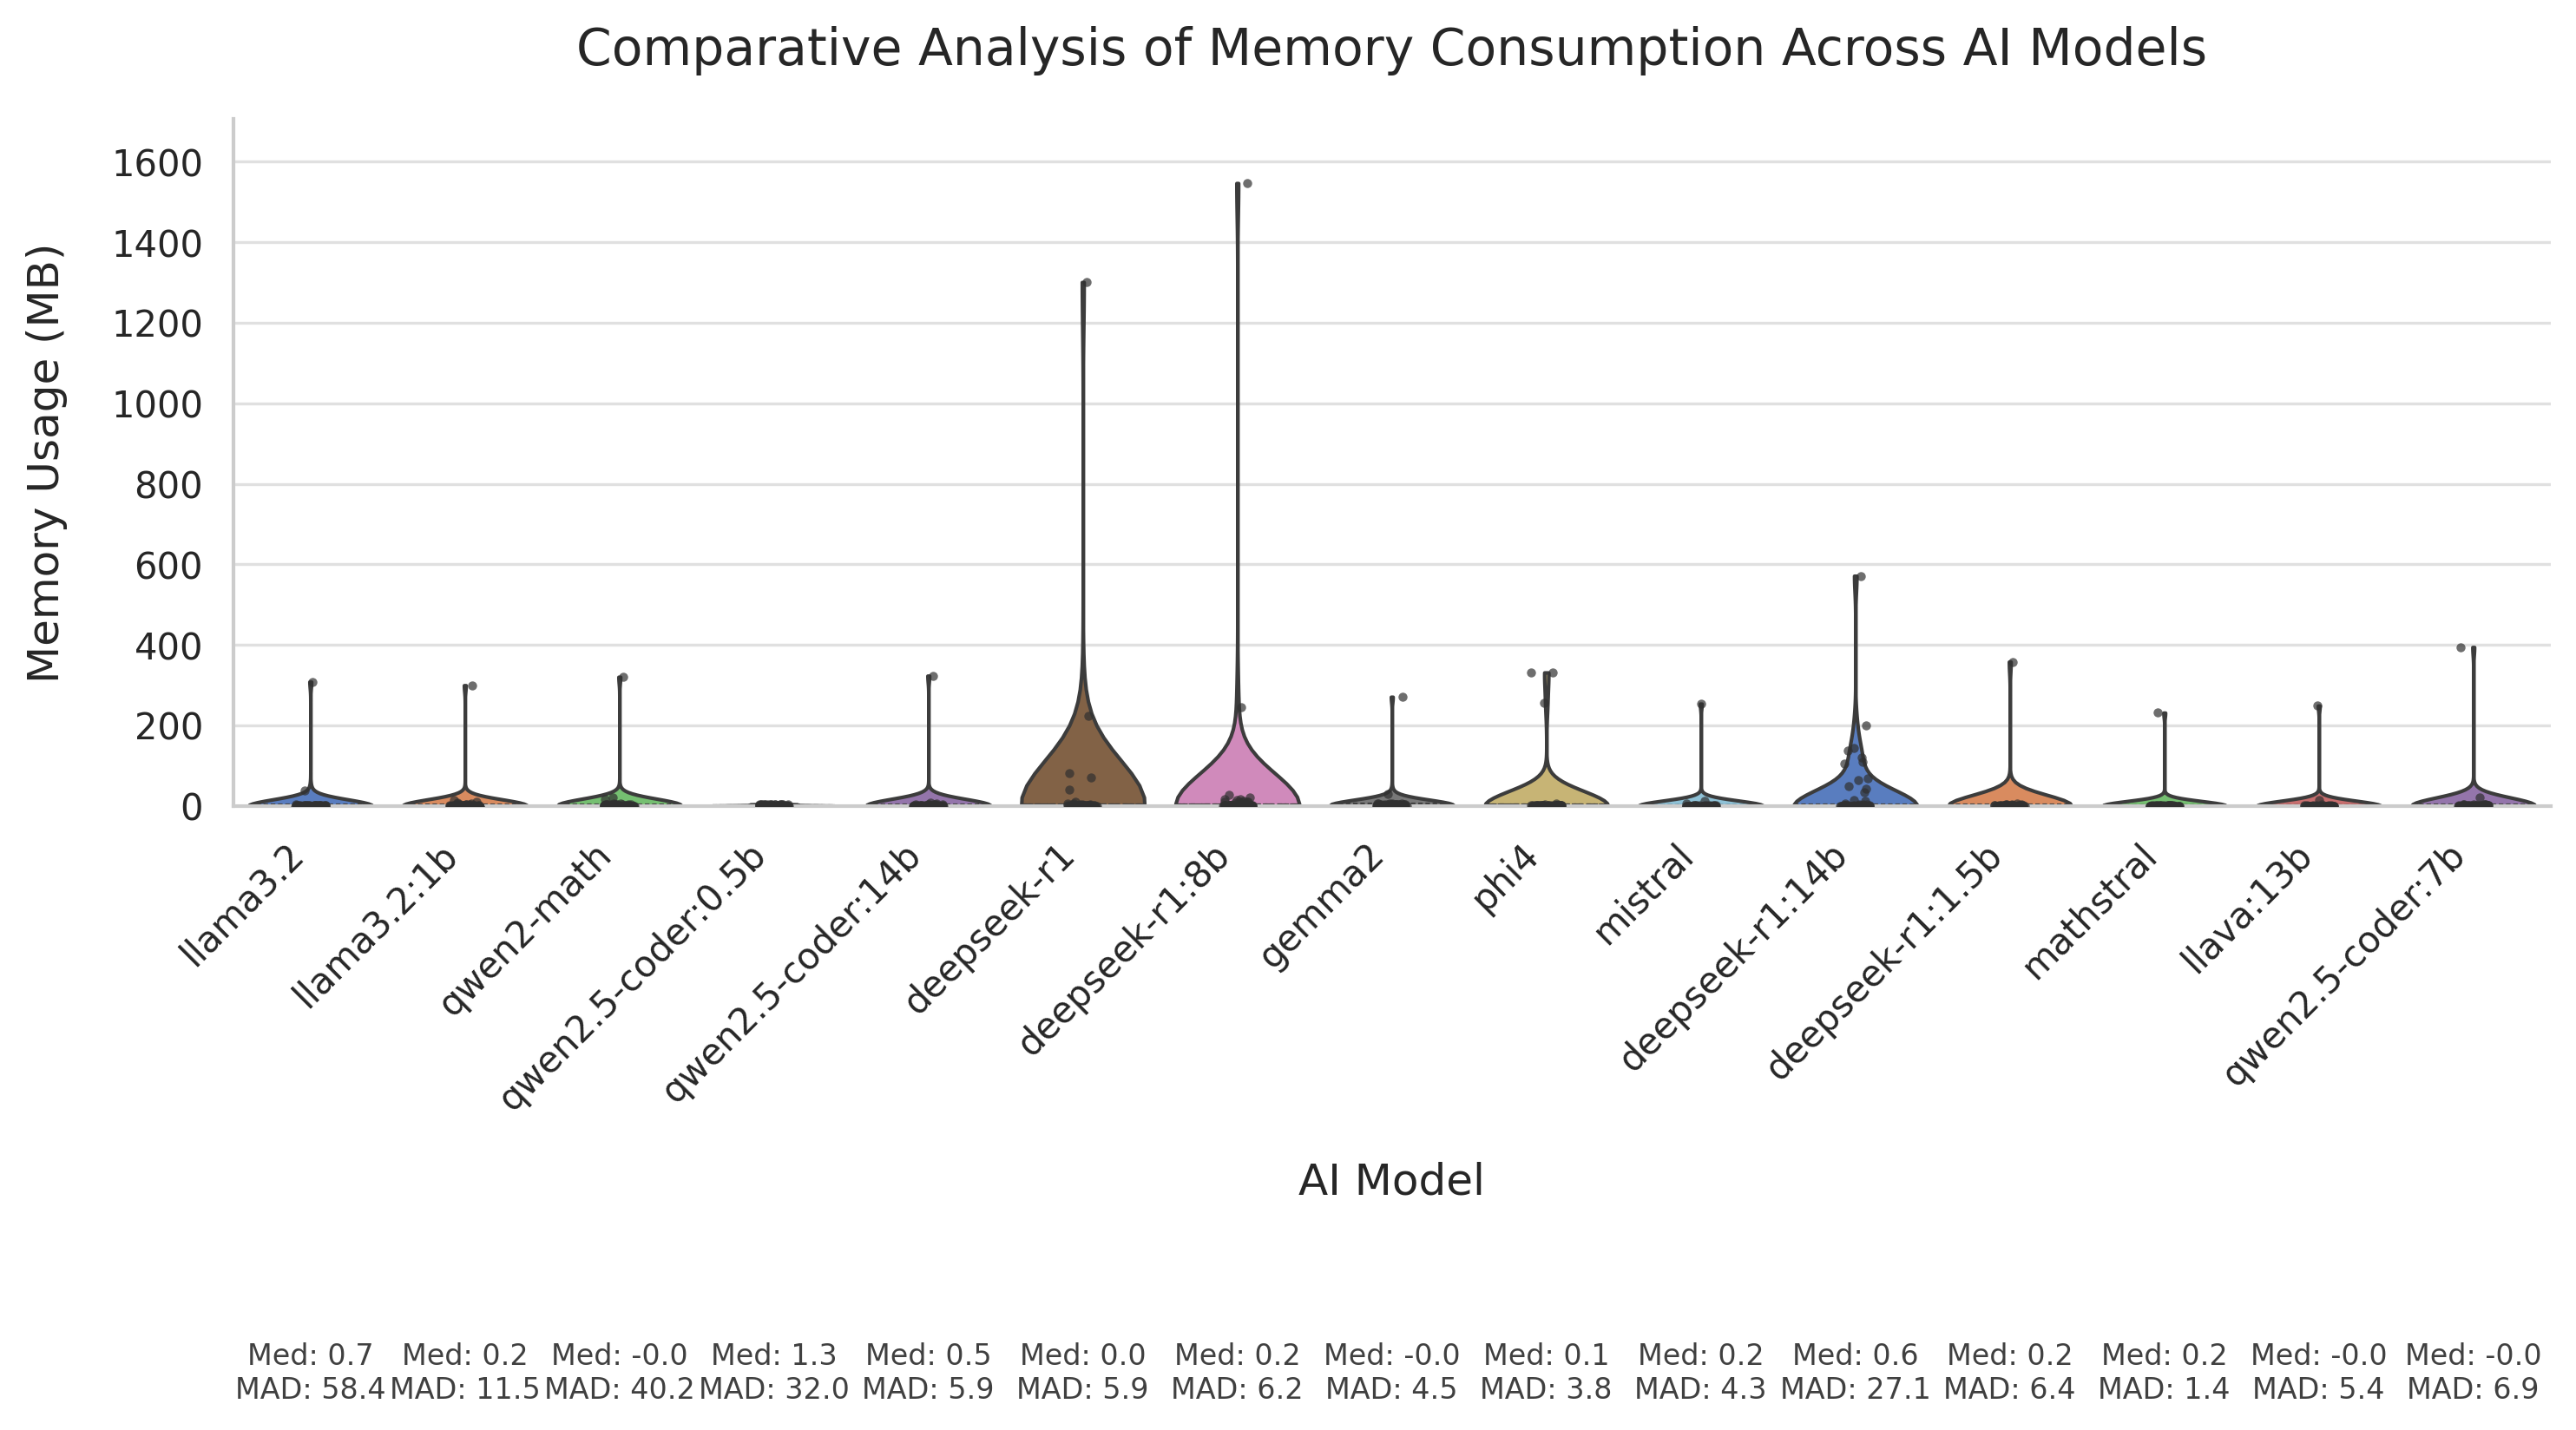
\includegraphics[width=0.9\columnwidth]{model_memory_usage_comparison.png}
        \caption{Memory Usage Comparison}
        \label{fig:memory-usage}
      \end{figure}
  \end{columns}
\end{frame}


\begin{frame}{Server}
  \begin{itemize}
    \item \textbf{Server Hardware:}
    %Bild???
      \begin{itemize}
        \item CPU: Intel Core i5.8600k
        \item GPU: NVIDA GeForce RTX 2060
        \item RAM: 16GB DDR4 
        \item Motherboard: H370 Chipset
        \item Power Supply: 500W BeQuiet
        \item Storage: 512GB NVMe SSDd
      \end{itemize}
    \item \textbf{Used Operating System:} The Server is running with the Ubuntu Server Operating System. The Operating System has been chosen due to the good cuda support. 

  \end{itemize}
\end{frame}

\begin{frame}{Server}
  \begin{itemize}
    \item \textbf{Networking:}
      \begin{itemize}
        \item Axios: Used for server requests 
        \item Tailscale: VPN tunnel used for secure remote access 
      \end{itemize}
    \item \textbf{Backup and Recovery:} Regular system backups have been made to avoid data loss.      
  \end{itemize}
\end{frame}

\begin{frame}{Flask Service}
  \begin{itemize}
    \item Flask as a Web Framework
    \item Architecture and Service Structure
    \item Restful Endpoints and Functionalities
    \item Deployment with Docker
  \end{itemize}
\end{frame}


\begin{frame}{Visual Studio Code Extension}
  \begin{itemize}
    % Bild !!!
    \item VS Code API / Typescript
    \item Server Request
    \item Integrated Chatbot
    \item Status Bar Item 
  \end{itemize}
\end{frame}

\begin{frame}{Operating System Market Share} 
  \begin{itemize}
    % Bilder !!!
    \item \textbf{Competitors:} Android, Microsoft Windows, Apple and Linux hold most of the market.
    \item  Bild
    \item \textbf{For Servers:} When looking at Server Operating Systems specifically The main Competitors are Red Hat and Microsoft.
    \item  Bild
  \end{itemize}
\end{frame}


\begin{frame}[plain]
  % Background HTL logo with transparency
  \begin{tikzpicture}[remember picture,overlay]
    \node[opacity=0.2] at (current page.center) 
      {
\includegraphics[width=0.6\paperwidth]{HTL-logo.jpeg}};
  \end{tikzpicture}
  
  \centering
  \vspace{1cm}
  \Huge Thank You for Your Attention!
\end{frame}

\end{document}
